%; whizzy chapter
% -initex iniptex -latex platex -format platex -bibtex jbibtex -fmt fmt
% 以上 whizzytex を使用する場合の設定。

%     Kansai Debian Meeting resources
%     Copyright (C) 2007 Takaya Yamashita
%     Thank you for Tokyo Debian Meeting resources

%     This program is free software; you can redistribute it and/or modify
%     it under the terms of the GNU General Public License as published by
%     the Free Software Foundation; either version 2 of the License, or
%     (at your option) any later version.

%     This program is distributed in the hope that it will be useful,
%     but WITHOUT ANY WARRANTY; without even the implied warranty of
%     MERCHANTABILITY or FITNESS FOR A PARTICULAR PURPOSE.  See the
%     GNU General Public License for more details.

%     You should have received a copy of the GNU General Public License
%     along with this program; if not, write to the Free Software
%     Foundation, Inc., 51 Franklin St, Fifth Floor, Boston, MA  02110-1301 USA

%  preview (shell-command (concat "evince " (replace-regexp-in-string "tex$" "pdf"(buffer-file-name)) "&"))
% 画像ファイルを処理するためにはebbを利用してboundingboxを作成。
%(shell-command "cd image200708; ebb *.png")

%%ここからヘッダ開始。

\documentclass[mingoth,a4paper]{jsarticle}
\usepackage{kansaimonthlyreport}
\usepackage[dvips]{xy}
\usepackage{ulem}

% 日付を定義する、毎月変わります。
\newcommand{\debmtgyear}{2012}
\newcommand{\debmtgdate}{23}
\newcommand{\debmtgmonth}{12}
\newcommand{\debmtgnumber}{67}

\begin{document}

\begin{titlepage}

% 毎月変更する部分、本文の末尾も修正することをわすれずに

 第\debmtgnumber{}回 関西 Debian 勉強会資料

\vspace{2cm}

\begin{center}
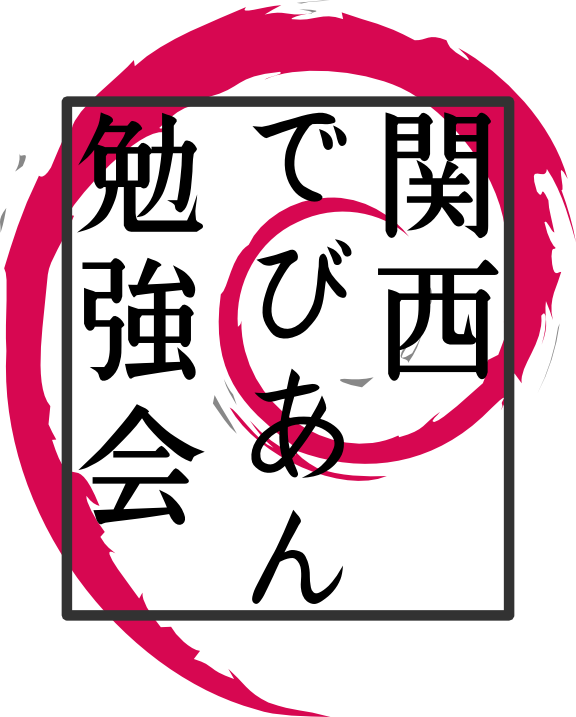
\includegraphics{image200802/kansaidebianlogo.png}
\end{center}

\begin{flushright}
\hfill{}関西 Debian 勉強会担当者 佐々木・倉敷・のがた・かわだ \\
\hfill{}\debmtgyear{}年\debmtgmonth{}月\debmtgdate{}日
\end{flushright}

\thispagestyle{empty}
\end{titlepage}

\dancersection{Introduction}{Debian JP}

\vspace{1em}

 関西Debian勉強会はDebian GNU/Linuxのさまざまなトピック
 (新しいパッケージ、Debian特有の機能の仕組、Debian界隈で起こった出来事、
 などなど)について話し合う会です。

 目的として次の三つを考えています。
 \begin{itemize}
  \item MLや掲示板ではなく、直接顔を合わせる事での情報交換の促進
  \item 定期的に集まれる場所
  \item 資料の作成
 \end{itemize}

 それでは、楽しい一時をお楽しみ下さい。

\newpage

\begin{minipage}[b]{0.2\hsize}
 {\rotatebox{90}{\fontsize{80}{80}
{\gt 関西 Debian 勉強会}}}
\end{minipage}
\begin{minipage}[b]{0.8\hsize}
\hrule
\vspace{2mm}
\hrule
\setcounter{tocdepth}{1}
\tableofcontents
\vspace{2mm}
\hrule
\end{minipage}

\dancersection{最近のDebian関係のイベント報告}{Debian JP}

\subsection{第 66 回関西 Debian 勉強会}

66 回目の関西 Debian 勉強会は 11 月 9 日、10 日に行なわれた関西オープンソース2012に出展しました。

インフォグラフィック、Wheezy DI Beta3 の DVD 配布とインストーラの実機展示、物販をブースで行ない、「Debian 7.0 "Wheezy" の紹介」と題してセミナー発表を行ないました。


\subsection{第 95 回東京エリア Debian 勉強会}
95 回目の東京エリア Debian 勉強会は 12 月 15 日に開催されました。

「im-config」、「2012年度東京エリアDebian勉強会の振り返り」、「日本におけるDFSGの求める自由と2012年改正著作権法」といった内容でした。

事前課題の各自の DFSG に関する理解から著作権、TPP と盛り上ったようです。im-config については資料に掲載されていませんのでご注意を。

\dancersection{事前課題}{Debian JP}

今回は以下の課題を出題しました.
\begin{screen}
  \begin{enumerate}
  \item 関西Debian勉強会で今年印象に残った話と来年聞きたい話を教えてください。
  \item DebianPolicy の6章に目を通しておいてください。
  \end{enumerate}
\end{screen}

参加者の皆さんの解答は以下の通りです。
\begin{multicols}{2}
%%%%%%%%%%%%%%%%%%%%%%%%%%%%%%%%%%%%%%%%%%%%%%%%%%%%%%%%%%%%%%%%%%%%%%%%
% 二段組ここから
%%%%%%%%%%%%%%%%%%%%%%%%%%%%%%%%%%%%%%%%%%%%%%%%%%%%%%%%%%%%%%%%%%%%%%%%
\begin{prework}{ 川江 }
  \begin{enumerate}
  \item 特にありません。
  \item 了解
  \end{enumerate}
\end{prework}\vfill

\begin{prework}{ 佐々木洋平 }
  \begin{enumerate}
  \item 大統一、かな。よくできたと思います. 来年度も是非やりたいですね。
  \item 了解です。
  \end{enumerate}
\end{prework}\vfill

\begin{prework}{ のがたじゅん }
  \begin{enumerate}
  \item 今年印象に残ったのは勉強会に入らないかもしれないけど大統一と、LDAP周りはあまり話しをする事がないから残ったかな。
    来年は、パッケージを久々に作ろうと思ったら浦島太郎状態だったので今どきのパッケージの作り方とか?
  \item わかりました。
  \end{enumerate}
\end{prework}\vfill

\begin{prework}{ かわだてつたろう }
  \begin{enumerate}
  \item 温泉合宿、大統一、Ralf さんの話しがよかったです。
    来年は月刊 Debian Policy と LDAP の話しの続きをやりたいですね。
  \end{enumerate}
\end{prework}\vfill

\begin{prework}{ cuzic }
  \begin{enumerate}
  \item 初参加なので、分かりません。。。Debian も初心者なんで。
  \item 当日までにやっておきます。。。
  \end{enumerate}
\end{prework}\vfill

\begin{prework}{ yyatsuo }
  \begin{enumerate}
  \item 前半はパッケージ系(やってみた)が多く、後半は LDAP などの認証系の話題が多かったのが印象的でした。
    他にも温泉合宿、大統一勉強会、Ralf さんの EDOS の話なんかがありましたね。\\
    来年は西田さんと酒井さんのパッケージの今後を見守りたいですね。
  \item 見ておきます
  \end{enumerate}
\end{prework}\vfill

\begin{prework}{ lurdan }
  \begin{enumerate}
  \item 温泉合宿と大統一がよかったですねー。
    あと、Debian Policy の輪読や複数の人が新たにパッケージ作成に挑戦、などなど新しい試みもあったなぁとか。
    来年は wheezy も出るはずなので、またサイクルを戻して初心者講座とかするのがいいのかなぁ。
  \item ざっくりと見ておきました
  \end{enumerate}
\end{prework}\vfill

\begin{prework}{ 大林 }
  \begin{enumerate}
  \item 今回初めて参加するので「特になし」ということで
  \end{enumerate}
\end{prework}\vfill

\begin{prework}{ ワチ マサタカ }
  \begin{enumerate}
  \item 初参加なので印象に残った話はわからないです。\\
    来年は、パッケージメンテナの人が仕事とどう両立させてるかを聞いてみたいです。
  \item 通しておきます。
  \end{enumerate}
\end{prework}\vfill

\begin{prework}{  清野陽一 }
  \begin{enumerate}
  \item あまり参加できなかったので…。来年はたくさん参加して色々な話を聞きたいです。
  \item はーい
  \end{enumerate}
\end{prework}\vfill

\begin{prework}{ 山城の国の住人 久保博 }
  \begin{enumerate}
  \item 今年印象に残った話
    \begin{description}
    \item[スクリプト言語 Konoha の Debianパッケージ化]\mbox{}
      Konoha がライセンスに関して混沌としていたのが衝撃的でした。
    \item[News from EDOS: finding outdated packages]\mbox{}
      パッケージ管理の問題がコンピュータ科学の研究テーマに
      なっていることに感銘を受けました。
    \item[Debian ではじめる Kerberos 認証]\mbox{}\\
      Active Directory 連係以外で Kerberos が使われていることや、
      今でも開発され続けているのが意外でした。
    \item[その他]\mbox{}\\
      翻訳について盛り上がったことが印象に残りました。
    \end{description}
  \item 来年聞きたい話
    \begin{itemize}
    \item wheezy への移行について
    \item samba4 とどうつき合っていけばいいか
    \item 開発に関すること
    \end{itemize}
\end{enumerate}
\end{prework}\vfill


\end{multicols}
%%%%%%%%%%%%%%%%%%%%%%%%%%%%%%%%%%%%%%%%%%%%%%%%%%%%%%%%%%%%%%%%%%%%%%%%
% 二段組ここまで
%%%%%%%%%%%%%%%%%%%%%%%%%%%%%%%%%%%%%%%%%%%%%%%%%%%%%%%%%%%%%%%%%%%%%%%%

\clearpage

\dancersection{Android端末(Asus Transformer TF201)へのDebianインストール奮闘記}{cuzic}

\subsection{はじめに}
\begin{itemize}
 \item cuzic
       \begin{itemize}
        \item きゅーじっく
        \item 親指シフトキーボード使い
              \begin{itemize}
               \item 親指シフト:濁音(が だ)、捨て仮名(ゃ っ)をすべて1打鍵で入力可能
               \item 親指シフトキーボードのために普段はWindowsを利用
              \end{itemize}
       \end{itemize}
 \item 最近の出来事
       \begin{itemize}
        \item Windows 8のタッチ対応のUltrabookが欲しい
              \begin{itemize}
               \item Ultrabook
               \item タッチパネル対応
               \item フルHD (1920x1080) の高画質
               \item まともな日本語キーボード
               \item D-Sub 15pin による出力が可能(プレゼン用)
              \end{itemize}
        \item お金がなくてなかなか買えない・・・
              \begin{itemize}
               \item Android端末 (Asus Transformer Prime)を所有
              \end{itemize}
        \item Android 端末でも十分開発できるようにLinux環境構築に挑戦
       \end{itemize}
\end{itemize}

\subsection{Asus Eee Pad Transformer Prime}
\begin{itemize}
 \item Eee Pad Transformer Prime (日本名 TF201)
       \begin{itemize}
        \item キーボード付きAndroidタブレット
        \item キーボードはバッテリーでもあり、駆動時間は最大18時間
        \item 実際、日帰り出張でもまったく問題なし
       \end{itemize}
 \item 外部メモリが 64GB もある
       \begin{itemize}
        \item 正直、Androidでは使いきれない…
        \item Linuxも入れちゃおう!!!
       \end{itemize}
\end{itemize}

\subsection{むかしむかし}
\begin{itemize}
 \item 実は、TF201を買ってすぐもLinux動作にチャレンジ
 \item ぜんぜんダメだった。
       \begin{itemize}
        \item いろんなキーが入力できない
              \begin{itemize}
               \item Ctrl、Alt、`(backtick)、@(atmark)
              \end{itemize}
        \item ほかにもいろいろあったはずだけど思い出せない…
       \end{itemize}
 \item ほかの方法も考えた
       \begin{itemize}
        \item AndroidとLinuxのデュアルブートとか
        \item もとの環境をつぶしてLinuxだけにするとか
        \item けど、できたらAndroidの中でアプリみたいな形でLinuxを動かしたい
       \end{itemize}
 \item 今回、再チャレンジ!
\end{itemize}

\subsection{まずは Ubuntu で試そうとしてみた}
\begin{itemize}
 \item まずは root 化する
       \begin{itemize}
        \item 基本。
        \item xda-developers.com \footnote{\url{http://forum.xda-developers.com/showthread.php?t=1706588}} からツールをダウンロードして実行
        \item bat を実行するとあとはうまくやってくれる
       \end{itemize}
\item Ubuntu Installer for Android
      \begin{itemize}
       \item google play \footnote{\url{https://play.google.com/store/apps/details?id=com.appbuilder.u14410p30729&hl=ja}} からダウンロードし、インストール
       \item このアプリは実は手順書だけ。自動インストールじゃない(汗)
       \item 3種類の Ubuntu イメージがある
             \begin{itemize}
              \item Full……Unity とかといっぱいの GUI プログラム
              \item Small…LXDE と Firefox などの基本的な GUIプログラム
              \item Core……GUI なし。基本的なコマンドのみ
             \end{itemize}
      \end{itemize}
\end{itemize}

\subsection{Ubuntu インストール(Full 編)}

\begin{itemize}
 \item まずは、Full 版イメージを試そうとしてみる
       \begin{itemize}
        \item UnityとかといっぱいのGUIプログラム(3.5GB相当)
       \end{itemize}
 \item ぜんぜんうまくいかず、挫折
       \begin{itemize}
        \item インストール編
              \begin{itemize}
               \item 大きすぎて、Androidからうまくダウンロードできない
               \item パソコンからダウンロードして、Androidに移動させる
              \end{itemize}
        \item 動作編
              \begin{itemize}
               \item Unity が重すぎて、うまく動かない orz
               \item そもそも、Firefoxがぜんぜん動かない
               \item LXDE をインストールしてみる。
               \item ほかもいろいろインストールしてみる。
                     \begin{itemize}
                      \item あっという間に容量上限(4GB)に達する
                     \end{itemize}
              \end{itemize}
        \item Small に変更して、再チャレンジしてみる。
       \end{itemize}
\end{itemize}

\subsection{Ubuntu インストール(small 編)}

\begin{itemize}
 \item Small 編
       \begin{itemize}
        \item LXDEとFirefox等の GUIプログラムつき
        \item 全体で 1.5 GBだから軽い
       \end{itemize}
 \item まずまずうまくいったが、やっぱ挫折
       \begin{itemize}
        \item うまくいった点
              \begin{itemize}
               \item LXDEはだいぶ軽い。ちゃんと動く。
               \item 開発環境構築関係についてはうまくいった
              \end{itemize}
        \item だけど…
              \begin{itemize}
               \item やっぱりFirefoxは動かない
               \item Chromiumも動かない
               \item Konquerorは動く
              \end{itemize}
       \end{itemize}
 \item タイムリーにLurdanさんと話した結果、Debianで再チャレンジすることに。
\end{itemize}

\subsection{Debian をインストール}
  \begin{itemize}
   \item Debian Kit for Android \footnote{\url{http://sven-ola.dyndns.org/repo/debian-kit-en.html}}を使ってインストールした
   \item インストール方法
         \begin{itemize}
          \item 基本的には手順に従うだけ
          \item Debian 6.0.6 (squeeze) をインストールしてみた。
          \item apt-get install andromize が重要
                \begin{itemize}
                 \item Android側に追随して /etc/resolv.conf を変更する
                \end{itemize}
         \end{itemize}
   \item 動作概要

   \begin{itemize}
    \item img ファイルを loopデバイスとしてマウント
    \item chroot せず、/ 以下に usr、var などが配備される
    \item VNCサーバを起動し、AndroidアプリのVNCクライアントから、DebianのX環境にアクセスする
   \end{itemize}
   \item 結果
         \begin{itemize}
          \item Firefox(iceweasel)もちゃんと動作した!
          \item ほかのいろんなのもまぁまぁ動いた
         \end{itemize}
  \end{itemize}

\subsection{容量を増やした}
\begin{itemize}
 \item Linuxが4GB(初期値)では足りない
       \begin{itemize}
        \item 10GBくらいはDebianに割当てたい
       \end{itemize}
 \item Windows PCのVirtualboxのUbuntuで下記手順を実施
\end{itemize}

\begin{commandline}
# virtualbox側で
nc -l 9000 > debianold.img
# asus transformer prime 側で
busybox nc virtualbox 9000 < /sdcard/debian.img
# virtualbox 側で
dd if=/dev/zero of=debiannew.img bs=1M count=0 seek=10240
mke2fs -F debiannew.img
mkdir debianold debiannew
sudo mount -o loop debianold.img debianold
sudo mount -o loop debiannew.img debiannew
rsync debianold/ debiannew
umount debianold; debiannew
# asus transformer prime 側で
busybox nc -l -p 9000 > /sdcard/debian.img
# virtualbox 側で
nc prime 9000 < debiannew.img
\end{commandline}

\subsection{ハマったところ}
\begin{itemize}
 \item 追加インストールが結構必要
       \begin{itemize}
        \item (例) sudo 、netcat
        \item Ubuntu にあるパッケージがDebianだと見つからない
              \begin{itemize}
               \item (例)leiningen(プログラミング言語clojure用の便利ツール)
              \end{itemize}
       \end{itemize}
 \item root だとネット接続可能なのに、自分で追加したユーザではネット接続不可
       \begin{itemize}
        \item 適切なグループへの追加が必要だったらしい。( Paranoid
              Network- ing
              \footnote{\url{http://elinux.org/Android_Security}} )
        \begin{commandline}
usermod -G inet,net\_raw,net\_admin cuzic
        \end{commandline}
       \end{itemize}
 \item /debian ディレクトリに直接ファイルを配置したが失敗
       \begin{itemize}
        \item loop デバイスとしてマウントせず、そのまま同居したかった
        \item /debian/\{usr,etc,varなど\} を置いてみた
        \item SDカードのファイルシステムがFAT32(?)でpermissionをうまく設定できず失敗=> loop デバイスの方法で利用し続けることにした。
       \end{itemize}
 \item Ctrl, Altがうまく使えない
       \begin{itemize}
        \item Emacsなどの利用において、致命的な問題
        \item AndroidのVNC Player側の問題
        \item 改変版のAndroid VNC Viewerを使うことで解決
        \item ※ ここ
              \footnote{\url{http://code.google.com/p/android-vnc-viewer/issues/detail?id=238}}
              の Comment 28 でコンパイル済みのバイナリを利用
       \end{itemize}
\end{itemize}

\subsection{まだできていないこと}
\begin{itemize}
 \item OpenOffice.org 、LibreOfficeの利用
      \begin{itemize}
       \item なんでか、 Impressをインストールできなかった
      \end{itemize}
 \item Caps lock、「半角/全角」、「無変換」、「変換」キーの利用
       \begin{itemize}
        \item VNCプレイヤー側の問題
        \item Android側ではキーイベントを拾えるみたい
        \item 無変換、変換が使えれば夢の 親指シフト化 が実現!
        \item Caps lockとCtrlを入れ替えたい
        \item 「半角/全角」をESCにしたい
       \end{itemize}
 \item Clojure開発環境での構築
       \begin{itemize}
        \item Ubuntu だと leiningen のパッケージがある
        \item Debian には leiningen のパッケージがない
       \end{itemize}
\end{itemize}

\subsection{まとめ}
\begin{itemize}
 \item Android タブレットでのDebian稼働は十分実用的
       \begin{itemize}
        \item ブラウザやエディタも十分動かせる
        \item 容量も十分なサイズでできる
        \item 一部のキー配列(Ctrl、ESC)が気になるくらい
        \item ちょっと動作はやっぱ遅い
       \end{itemize}
 \item Android 環境とDebian環境を同時実行できるのも便利
       \begin{itemize}
        \item ブラウザはAndroidのブラウザで
        \item 開発はDebianのvi/emacsで
       \end{itemize}
 \item Android タブレットの長所を持つ開発環境の誕生
       \begin{itemize}
        \item バッテリーが長持ち、薄くて軽い
       \end{itemize}
 \item けど、ほんとうは新しいノートパソコンが欲しい
       \begin{itemize}
        \item お金がないから、AndroidタブレットのDebian化で我慢
       \end{itemize}
\end{itemize}

\clearpage

\dancersection{月刊 Debian Policy「パッケージ管理スクリプトとインストールの手順」}{かわだ てつたろう}

月刊 Debian Policy、今回読むのは第 6 章の「パッケージ管理スクリプトとインストールの手順」です。
この章ではパッケージをインストール、アップグレード、削除する際にパッケージ管理システムが走らせるスクリプトとその手順について説明されています。

さて、事前課題で内容は読んで理解していただいていると思いますのでざっと内容をみていきましょう。

\subsection{パッケージ管理スクリプト}
パッケージ管理スクリプトは次の 4 つの制御情報ファイルで、パッケージの一部として供給されます。

\begin{itemize}
\item preinst
\item postinst
\item prerm
\item postrm
\end{itemize}



\subsubsection{ファイル構成}
パッケージ管理スクリプトは実行可能ファイルでなければならず、ファイルのパーミッションは、誰でも読むことと実行可能でなければならないが誰でも書き込み可能ではいけない、{\tt 755} でなければいけません。
また、スクリプトであることが推奨されており、その場合は {\tt \#!} (shebang) で始まってなければなりません。

\subsubsection{終了ステータス}
パッケージ管理システムは終了ステータスコードを参照するので正しく終了ステータスコードを返すことが重要です。
処理が成功すれば 0 を、失敗すれば 0 以外を返さなければなりません。0 以外のステータスコードが返された場合、パッケージ管理システムはエラーと判断し以降の処理を停止します。

パッケージ管理スクリプトがシェルスクリプトなら常に {\it set -e} を使用する必要があります。

\subsubsection{PATH 環境変数}
{\tt PATH} 環境変数内から見つかることが期待できるプログラムは絶対パスで呼びだすべきではありません。
また、{\tt PATH} 環境変数はリセットすべきではありませんが、前後に付け加えることはかまいません。

\subsubsection{再入結果の同一性}
パッケージ管理スクリプトは、一度成功した処理を何度呼び出しても無害でなければならず、
失敗や中断した処理を再度呼び出しても前回の残された状態から実行しなければなりません。
いずれにせよ全ての処理が成功した場合にはパッケージ管理スクリプトは成功ステータスで終了しなければなりません。

これは、ひどく壊れたパッケージが残らないようにするためにとても重要です。

\subsubsection{パッケージ管理スクリプトからのターミナルの制御}
パッケージ管理スクリプトは、制御端末がある状態での実行が保証されていません。
ユーザとの対話ができない場合がありますので、非対話型で処理できるようにしなければなりません。

どうしても対話が必要な場合(優先順位が高く、妥当な標準回答がないなど)に制御端末が無ければパッケージ管理スクリプトは異常終了してもかまいません。
ただ、できるだけこのような状況は避けるべきです。たいていの場合、パッケージのバグと判断されます。

{\tt debconf} を用いる場合はの詳細は「3.9.1 メンテナスクリプト中のプロンプト使用について」を参照してください。


\subsection{パッケージ管理スクリプトの呼ばれ方のまとめ}
パッケージ管理スクリプトがそれぞれ呼ばれるタイミングをおおまかにいうと次のようになります。

\begin{itemize}
\item preinst  … パッケージ展開前
\item postinst … パッケージ展開後
\item prerm    … パッケージ削除前
\item postrm   … パッケージ削除後
\end{itemize}

ここからは、パッケージ管理スクリプトのすべての呼ばれ方と、呼ばれる際に依存して良い機能についてのまとめです。
{\it new-} はインストール/更新/ダウングレード対象の新バージョンのパッケージから呼ばれるもの、
{\it old-} は更新/ダウングレードされる対象の旧バージョンのパッケージから呼ばれるものです。


\subsubsection{preinst}

\begin{itemize}
\item {\it new-preinst} install
\item {\it new-preinst} install {\it old-version}
\item {\it new-preinst} upgrade {\it old-version}
  \begin{itemize}
  \item パッケージは展開前
  \item essential パッケージと Pre-Depends パッケージのファイルのみがある
  \item Pre-Depends パッケージは展開された直後か Half-Configured の可能性がある
  \end{itemize}
\end{itemize}

\begin{itemize}
\item {\it old-preinst} abort-upgrade {\it new-version}
  \begin{itemize}
  \item アップグレードに失敗した場合に呼ばれる
  \item 展開されたファイルに依存してはいけない
  \item パッケージの依存関係は満たされていないかもしれない
  \item Pre-Depends は上記と同様
  \end{itemize}
\end{itemize}


\clearpage

\subsubsection{postinst}

\begin{itemize}
\item {\it postinst} configuire {\it most-recently-configured-version}
  \begin{itemize}
  \item パッケージと依存パッケージのファイルは展開されている
  \item 巡回依存関係になければ依存パッケージは設定されている
  \end{itemize}
\end{itemize}

\begin{itemize}
\item {\it old-postinst} abort-upgrade {\it new-version}
\item {\it conflictor's-postinst} abort-remove in-favour {\it package} {\it new-version}
\item {\it postinst} abort-remove
\item {\it deconfigured's-postinst} abort-deconfigure in-favour {\it failed-install-package} {\it version} [removing {\it conflicting-package} {\it version}]
  \begin{itemize}
  \item パッケージのファイルは展開されている
  \item 依存する全てのパッケージは少くとも Half-Installed 状態、完全に展開されていないこともある
  \item 依存関係が必要となる処理は実行するべきである、依存関係が満たされていないたいていの場合 {\tt postinst} を異常終了させるのがエラー処理を考慮すると適切な処理である
  \end{itemize}
\end{itemize}


\subsubsection{prerm}

\begin{itemize}
\item {\it prerm} remove
\item {\it old-prerm} upgrade {\it new-version}
\item {\it conflictor's-prerm} remove in-favour {\it package} {\it new-version}
\item {\it deconfigured's-prerm} deconfigure in-favour {\it package-being-installed} {\it version} [removing {\it conflicting-package} {\it version}]
  \begin{itemize}
  \item パッケージは Half-Installed 状態
  \item 依存する全てのパッケージは少くとも Half-Installed 状態、完全に展開されていないエラー状態なこともある
  \end{itemize}
\end{itemize}

\begin{itemize}
\item {\it new-prerm} failed-upgrade {\it old-version}
  \begin{itemize}
  \item {\it prerm} upgrade が失敗した際に呼び出される
  \item 新しいパッケージは展開されておらず {\it preinst} upgrade と同じ制約下にある
  \end{itemize}
\end{itemize}


\subsubsection{postrm}

\begin{itemize}
\item {\it postrm} remove
\item {\it postrm} purge
\item {\it old-postrm} upgrade {\it new-version}
\item {\it disappearer's-postrm} disappear {\it overwriter} {\it overwriter-version}
  \begin{itemize}
  \item パッケージのファイルが削除、置き換えられた後に呼び出される
  \item 依存関係は考慮されていない状態
  \item essential パッケージのみに依存した処理とすること
  \item 依存関係が必要な処理で依存関係が満たされていない場合はすべて丁寧に処理を飛ばすようにしなければいけない
  \end{itemize}
\end{itemize}


\begin{itemize}
\item {\it new-postrm} failed-upgrade {\it old-version}
  \begin{itemize}
  \item 古いパッケージの {\it postrm} upgrade が失敗した場合に呼ばれる
  \item 新しいパッケージのファイルは展開されているが、essential パッケージと Pre-Depends パッケージのみへ依存できる
  \end{itemize}
\end{itemize}

\begin{itemize}
\item {\it new-postrm} abort-install
\item {\it new-postrm} abort-install {\it old-version}
\item {\it new-postrm} abort-upgrade {\it old-version}
  \begin{itemize}
  \item preinst が失敗したエラー処理の一環で新しいパッケージを展開する前に呼ばれる
  \item preinst と同じ制約下
  \end{itemize}
\end{itemize}



\subsection{各段階の詳細}
ここでは流れを掴みやすくするためエラー処理を省いたパッケージのインストール、設定、削除の詳細をみていきます。
エラー処理について元のポリシーに記述されていますので参照してください。


\subsubsection{インストール時とアップグレート時のパッケージの展開段階の詳細}
\begin{enumerate}

\item インストールされたパッケージがある場合
  \begin{itemize}
  \item {\it old-prerm} upgrade {\it new-version}
  \end{itemize}

\item 衝突するパッケージが削除されようとしているか、壊れたパッケージ(Breaks のため)の場合
  \begin{enumerate}
  \item --auto-deconfigure が指定されていた場合
    \begin{enumerate}
    \item Breaks で設定破棄されるパッケージに対して
      \begin{itemize}
      \item {\it deconfigured's-prerm} deconfigure in-favour {\it package-being-installed} {\it version}
      \end{itemize}
    \item 削除されようとしている衝突するパッケージが依存するパッケージに対して
      \begin{itemize}
      \item {\it deconfigured's-prerm} deconfigure in-favour {\it package-being-installed} {\it version} removing {\it conflicting-package} {\it version}
      \end{itemize}
    \end{enumerate}
  \item 衝突して削除されるパッケージに対して
    \begin{itemize}
    \item {\it conflictor's-prerm} remove in-favour {\it package} {\it new-version}
    \end{itemize}
  \end{enumerate}

\item
  \begin{enumerate}
  \item アップグレードの場合
    \begin{itemize}
    \item {\it new-preinst} upgrade {\it old-version}
    \end{itemize}
  \item 設定ファイルが残っていた場合
    \begin{itemize}
    \item {\it new-preinst} install {\it old-version}
    \end{itemize}
  \item それ以外(purge された状態)の場合
    \begin{itemize}
    \item {\it new-preinst} install
    \end{itemize}
  \end{enumerate}

\item 新しいパッケージのファイルを展開し上書き(古いファイルはバックアップされる)
  \begin{itemize}
  \item Replace 指定なしに既にシステムにある他のパッケージのファイルを含んでいるとエラー
  \item 同じく Replace 指定なしに他のパッケージのディレクトリと同名のファイルやディレクトリ以外のものを含んでいるとエラー
    \begin{itemize}
    \item --force-overwrite-dir でエラーを無効にできるが、勧められない
    \item ディレクトリがシンボリックリンクで置き換えられることはないし、逆もまたない
    \end{itemize}
  \end{itemize}

\item アップグレードされた場合
  \begin{itemize}
  \item {\it old-postrm} upgrade {\it new-version}
  \end{itemize}

{\underline {\Large ここが戻れなくなるポイント}}


\item 新しいパッケージで使われなくなった古いパッケージのファイルを削除

\item 新しいファイルリストに更新

\item 新しいパッケージ管理スクリプトに更新

\item 全てのファイルが上書きされ、要求も依存もされなくなったパッケージがあった場合(削除されたとみなされ次の処理が行われる)
  \begin{enumerate}
  \item {\it disappearer's-postrm} disappear {\it overwriter} {\it overwriter-version}
  \item パッケージ管理スクリプトの削除
  \item パッケージがインストールされていない状態となる。(conffile は無視され、prerm も呼び出されない)
  \end{enumerate}

\item 新しいパッケージのファイルが他のパッケージのファイルリストに記されていれば、それらをリストから削除

\item バックアップファイルを削除

\item 新しいパッケージを unpacked 状態にする\\
{\underline {\Large もう一つの戻れなくなるポイント}}

\item 衝突するパッケージがあればそれらの削除処理へ

\end{enumerate}

\subsubsection{設定の詳細}
\begin{enumerate}
\item conffile を更新して
  \begin{itemize}
  \item {\it postinst} configure {\it most-recently-configured-version}
  \end{itemize}
  エラーが起こっても回復処理は行なわれず Failed Config 状態になる
\end{enumerate}


\subsubsection{削除と設定の完全削除の詳細}
\begin{enumerate}
\item {\it prerm} remove

\item パッケージのファイルを削除(conffile を除く)

\item {\it postrm} remove

\item postrm を除く全パッケージ管理スクリプトの削除\\
  purge でなければここで終了。purge でなくても postrm と conffile がなければ purge と同じ状態になる。

\item conffile とバックアップファイルを削除

\item {\it postrm} purge

\item パッケージのファイルリストを削除(postrm もここで削除)

\end{enumerate}


\subsection{最後に}
次回の月刊 Debian Policy は $\cdots$
\footnote{今日担当者が決まるかもしれません(佐々木)}。

\clearpage

\dancersection{2012年の振り返りと2013年の企画}{佐々木洋平/Debian JP Project}

今月が 2012 年最後の関西 Debian 勉強会になります。
初回が 2007 年 3 月ということで、今年で 6 年目になりますね。
今年は定例となっている OpenSource 関連のイベントへの参加だけではなく
「大統一Debian勉強会」を開催することができたのが大きな収穫だと思っています。

\subsection{勉強会全体について}

\subsubsection{月刊Debian Policy}
今年は「月刊物をなんかやってみないか?」ということで「月刊 Debian Policy」を始めてみました。
Debian Policy Manual, version 3.9.1 の日本語訳は Debian JP Project によって公開されています
\footnote{
  \texttt{http://www.debian.or.jp/community/devel/debian-policy-ja/policy.ja.html/}
}。「月刊 Debian Policy」では、
最新の Debian Policy Manual
\footnote{
  \texttt{http://www.debian.org/doc/debian-policy/}\newline
  現時点での最新版は 3.9.4.0, 2012-09-19
} を読み進めて勉強しながら、
現在公開されている日本語訳と突き合わせつつ、
(あわよくば)これを更新したいと考えています。
「Debian Policy Manual を勉強する」という目的は毎回の勉強会で非常に上手く進んでいると思います。
今後も進めて行きたいと思いますが、如何でしょうか。

\subsubsection{翻訳ネタ}

今年後半の関西Debian勉強会では「翻訳」に関する発表が幾つか行なわれました。
「翻訳」されて母国語で文書が読めることは、
ソフトウェアの普及やコミュニティの参加への敷居を下げるという点で、非常に重要です。
Debian JP では(不幸な事に)、作業プロセスが不透明であったり、
幾つかの(非常に重要な)翻訳作業が属人化している、という問題もあります。
今年の勉強会でせっかく盛り上がりつつある「翻訳熱」を冷ますことなく、
今後はなんらかの改善が行なわれると良いかな、と思っています。

\subsubsection{その他, 定例ネタ}

毎回のセッションについてですが、
今年は「パッケージ作成」や「BTS」に関する題材として「t-code」「Konoha」に関するお話を複数回にわたって発表して頂きました。
具体的に弄りたいパッケージがあると、(発表者のモチベーションが違うのか)非常に良い勉強会になった気がします。
来年は Wheezy がリリースされることですし、
定番のネタ(Debianの入門的なお話、ライセンス、パッケージ作成、BTS)などの題材に加えて、
「Wheezy から始める Debian 環境」みたいなお話もあったら良いかな、と考えています。
昨年は案が出たけで結局実施できなかった「インストール大会」のような初心者講習もやってみたい所ですね。

\subsection{運営}

運営に関しては、今年の(特に後半は)河田さんの獅子奮迅の活躍により勉強会が開催できていました。
運営側が多忙となってしまうのはある程度しかたない(かもしれない)ですが、
今後はもう少し個人の負担を減らしつつ開催していきたいと考えています。

\subsection{イベント/NM申請}

イベント参加については、OSC Kansai@Kyoto, KOF 2012 に参加しました。
勉強会から fork した GPG キーサインパーティも毎回実施されています。今後も継続して参加する予定です。
%
また、1月には関西初の「Debian 温泉合宿」が、6月には東京エリアDebian勉強会と合同で「大統一Debian勉強会」を開催しました。
これらのイベントは今後も継続して実施する予定です。

Debian 開発者への道、として佐々木と倉敷さんの二人が NM プロセスにて DD になるための申請中です。
今後も NM プロセスに挑む参加者や Debian Maintainer となって精力的にパッケージを開発/更新する人が増えると良いですね。

\subsection{開催実績}

関西Debian勉強会の出席状況を確認してみましょう。グラフで見る
と\fgref{fig:kansaipeoplechart}になります。また、毎回の参加者の人数とその
際のトピックを \tbref{tab:count2012kansai} にまとめました。グラフ中の黒線
は参加人数、赤線は1年の移動平均です。参加人数が$0$となっているところは人
数が集計されていないor開催されなかった月です。

Debian勉強会申し込みシステムを使用するようになり、事前課題を設定すること
も多くなりました。また、アンケートシステムも稼動するようになるでしょうか
ら、今後は事前課題と事後課題のグラフを追加しようと思っています。
%
\begin{figure}[h]
  \begin{center}
    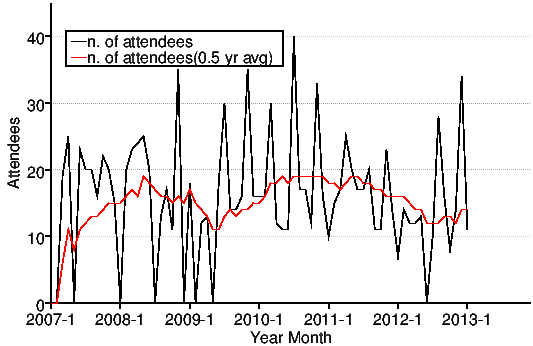
\includegraphics[width=.6\hsize]{image201212/memberanalysis/kansai.png}
  \end{center}
  \caption{関西の参加人数推移(参加人数と6ヶ月移動平均)}
  \label{fig:kansaipeoplechart}
\end{figure}

%\pagebreak

\begin{table}
  \begin{minipage}{.5\linewidth}
  \caption{関西Debian勉強会の参加人数とトピック(2007-2008年)}
  \begin{center}
    \begin{tabular}{|l|c|p{10em}|}
      \hline
                 & 参加人数 & 内容 \\
      \hline
      2007年3月  & 19       & 開催にあたり \\
      2007年4月  & 25       & goodbye、youtube、プロジェクトトラッカー\\
      2007年6月  & 23       & 社会契約、テーマ、debian/rules、bugreport\\
      2007年7月  & 20前後   & OSC-Kansai \\
      2007年8月  & 20       & Inkscape、patch、dpatch\\
      2007年9月  & 16       & ライブラリ、翻訳、debtorrent\\
      2007年10月 & 22       & 日本語入力、SPAMフィルタ\\
      2007年11月 & 20前後   & KOF \\
      2007年12月 & 15       & 忘年会、iPod touch\\
      \hline
      \hline
                 & 参加人数 & 内容 \\
      \hline
      2008年2月  & 20       & PC Cluster, GIS, \TeX \\
      2008年3月  & 23       & bug report, developer corner, GPG \\
      2008年4月  & 24       & coLinux, Debian GNU/kFreeBSD, sid \\
      2008年5月  & 25       & ipv6, emacs, ustream.tv\\
      2008年6月  & 20       & pbuilder, hotplug, ssl\\
      2008年8月  & 13       & coLinux \\
      2008年9月  & 17       & debian mentors, ubiquity, DFSG\\
      2008年10月 & 11       & cdbs,cdn.debian.or.jp \\
      2008年11月 & 35       & KOF \\
      2008年12月 & ?        & TeX資料作成ハンズオン\\
      \hline
    \end{tabular}
  \end{center}
\end{minipage}
\pagebreak
\begin{minipage}{.5\linewidth}
  \begin{center}
    \caption{関西Debian勉強会の参加人数とトピック(2009-2010)}
    \begin{tabular}{|l|c|p{10em}|}
      \hline
                 & 参加人数 & 内容 \\
      \hline
      2009年1月  & 18       & DMCK, LT \\
      2009年3月  & 12       & Git \\
      2009年4月  & 13       & Installing sid, Mancoosi, keysign \\
      2009年6月  & 18       & Debian Live, bash\\
      2009年7月  & 30?      & OSC2009Kansai \\
      2009年8月  & 14       & DDTSS, lintian \\
      2009年9月  & 14       & reportbug, debian mentors\\
      2009年10月 & 16       & gdb, packaging \\
      2009年11月 & 35       & KOF2009 \\
      2009年12月 & 16       & GPS program, OpenStreetMap \\
      \hline
      \hline
                 & 参加人数 & 内容 \\
      \hline
      2010年1月  & 16       & Xen, 2010年企画 \\
      2010年2月  & 16       & レンタルサーバでの利用, GAE \\
      2010年3月  & 30?      & OSC2010Kobe \\
      2010年4月  & 12       & デスクトップ環境, 正規表現 \\
      2010年5月  & 11       & ubuntu, squeeze \\
      2010年6月  & 11       & debhelper7, cdbs, puppet \\
      2010年7月  & 40?      & OSC2010Kyoto \\
      2010年8月  & 17       & emdebian, kFreeBSD \\
      2010年9月  & 17       & タイルWM \\
      2010年10月 & 12       & initramfs, debian live \\
      2010年11月 & 33       & KOF2010 \\
      2010年12月 & 14       & Proxmox, annual review \\
      \hline
    \end{tabular}
  \end{center}
\end{minipage}
\end{table}
\pagebreak
\begin{table}
%  \begin{minipage}{.5\linewidth}
    \caption{関西Debian勉強会の参加人数とトピック(2011)}
    \begin{center}
      %\begin{tabular}{|l|c|p{10em}|}
      \begin{tabular}{|l|c|l|}
        \hline
        開催年月  & 参加人数 & 内容 \\
        \hline
        2011年1月 &10        & BTS, Debian GNU/kFreeBSD\\
        2011年2月 &15        & pbuilder, Squeezeリリースパーティ\\
        2011年3月 &17        & ライセンス, Debianのドキュメント関連\\
        2011年4月 &25        & OSC 2011 Kansai @ Kobe, GPG キーサインパーティ \\
        2011年5月 &20        & vi, dpkg \\
        2011年6月 &17        & IPv6, vcs-buildpackage{svn, git}\\
        2011年7月 &17        & OSC 2011 Kansai @ Kyoto, GPG キーサインパーティ\\
        2011年8月 &20        & Debianパッケージ作成ハンズオン\\
        2011年9月 &11        & vcs-buildpackage{bzr, git}\\
        2011年10月&11        & Emacs, vim の拡張のDebianパッケージ, 翻訳\\
        2011年11月&23        & KOF 2011\\
        2011年12月&13        & NMプロセス, BTS\\
        \hline
      \end{tabular}
    \end{center}
%  \end{minipage}
%  \begin{minipage}{.5\linewidth}
    \caption{関西Debian勉強会の参加人数とトピック(2012)}
    \label{tab:count2012kansai}
    \begin{center}
%      \begin{tabular}{|l|c|p{10em}|}
      \begin{tabular}{|l|c|l|}
        \hline
        開催年月  & 参加人数 & 内容 \\
        \hline
        2012年1月 & 7        & Debian温泉合宿 \\
        2012年2月 &14        & autofs+pam\_chroot, t-codeその1, 月刊Debian Policy その1 \\
        2012年3月 &12        & 新年度スケジューリング, Konohaその1, t-codeその2, 月刊Debian Policy その2 \\
        2012年4月 &12        & フリーソフトウェアと著作権, Konohaその2, 月刊Debian Policy その3 \\
        2012年5月 &13        & DebianとLDAP(頓挫), ITP入門, 月刊Debian Policy その4 \\
        2012年6月 & -        & 大統一Debian勉強会 \\
        2012年7月 &10        & DebianとLDAPその1, 大統一Debian勉強会報告, 月刊Debian Policy その5 \\
        2012年8月 &28        & OSC 2012 Kansai @ Kyoto, GPG キーサインパーティ\\
        2012年8月 &16        & DebianとKerberos, News from EDOS \\
        2012年9月 & 8        & clang によるパッケージビルド, 月刊Debian Policy その6 \\
        2012年10月&14        & 翻訳環境構築, DSAの舞台裏\\
        2012年11月&34        & KOF 2012\\
        2012年12月&12        & Debian on Android, 月刊Debian Policy その7 \\
        \hline
      \end{tabular}
    \end{center}
%  \end{minipage}
\end{table}

\clearpage

\dancersection{今後の予定}{Debian JP}

\subsection{関西 Debian 勉強会}

次回、第 68 回関西 Debian 勉強会は 1 月 27 日(日)に国際奈良学セミナーハウスで行ないます。
内容は今日決まる予定ですので、以下の欄にしっかりとメモを取っておいて下さい。
\begin{screen}
  \vspace{5em}
\end{screen}

\subsection{東京エリア Debian 勉強会}
1 月 19 日(土)に 96 回目の東京エリア Debian 勉強会が開催されます。

% 冊子にするために、4の倍数にする必要がある。
% そのための調整
\dancersection{メモ}{}
\mbox{}\newpage
\mbox{}\newpage

\printindex
 \cleartooddpage

 \begin{minipage}[b]{0.2\hsize}
  \rotatebox{90}{\fontsize{80}{80} {\gt 関西 Debian 勉強会} }
 \end{minipage}
 \begin{minipage}[b]{0.8\hsize}

 \vspace*{15cm}
 \rule{\hsize}{1mm}
 \vspace{2mm}
 
\includegraphics[width=2cm]{image200502/openlogo-nd.eps}
 \noindent \Large \bf Debian 勉強会資料\\ \\
 \noindent \normalfont \debmtgyear{}年\debmtgmonth{}月\debmtgdate{}日 \hspace{5mm}  初版第1刷発行\\
 \noindent \normalfont 関西 Debian 勉強会 (編集・印刷・発行)\\
 \rule{\hsize}{1mm}
 \end{minipage}

\end{document}
